\documentclass[14pt,a4paper]{extarticle}
\usepackage[utf8]{inputenc}
\usepackage[T2A]{fontenc}
\usepackage[english,russian]{babel}
%\usepackage{fontspec}
%\setmainfont{Times New Roman} 
\usepackage[unicode]{hyperref}
\usepackage[left=2cm,right=1cm, top=2cm, bottom=2cm]{geometry}
\linespread{1.5}
\usepackage{indentfirst}
\usepackage{amssymb}
\usepackage{cmap}
\usepackage[]{graphicx}
\usepackage{hyperref}
\usepackage{array}
\usepackage{wrapfig}
\usepackage{longtable}
\usepackage{verbatim}
\usepackage{enumitem}
\usepackage{amsmath}
\usepackage{float}
\usepackage{mathtools}
\usepackage{icomma}
\usepackage{caption}
\captionsetup{labelsep=period}
\usepackage{xcolor}
\usepackage{animate}
%\numberwithin{equ`tion}{section}
\newcommand{\ten}[1]{\cdot 10^{#1}}
\hypersetup{
	colorlinks,
	citecolor=black,
	filecolor=black,
	linkcolor=black,
	urlcolor=blue
}

\usepackage{pdfpages}
\newcommand{\whr}{\text{, где}}
\newcommand{\razm}[1]{\hspace{1ex} \ensuremath{\left[\text{#1}\right]}}
\newcommand{\rbf}[1]{\textbf{\ref{#1}}}
\newcommand{\refris}[1]{рис. \rbf{#1}}
\newcommand{\prf}[1]{стр. \textbf{\pageref{#1}}}
\newenvironment{aleq}{\begin{equation}\begin{aligned}}{\end{aligned}\end{equation}}
\renewcommand{\geq}{\geqslant}
\renewcommand{\leq}{\leqslant}
\newcommand{\rt}[1]{_\text{#1}}
\newcommand{\mm}{\razm{мм}}
\newcommand{\ris}[1]{рис. \rbf{#1}}
\renewcommand{\phi}{\varphi}
\renewcommand{\epsilon}{\varepsilon}

\newcommand{\an}[2]{a_{#1}\cos \left({#2}\frac{2\pi x}{P}\right)}
\newcommand{\bn}[2]{b_{#1}\sin \left({#2}\frac{2\pi x}{P}\right)}
\newcommand{\mtrig}[2]{\frac{2}{{#2}\pi}{#1}\left({#2}\frac{2\pi x}{P}\right)}
\author{Максим Зотов}
\title{МТ11-62Б}
\date{Вариант  5 (10)}
\begin{document}
\maketitle
\tableofcontents
\pagebreak
\section{Заданные условия}
\begin{center}
\begin{tabular}{cccc}
	Линейный размер окна &W & 3 &\razm{мкм}\\
	Микрозазор &z & 1,186662 &\razm{мкм}\\
	Длина волны актиничного излучения&$\lambda$ & 0.24 &\razm{мкм}\\
\end{tabular}
\end{center}
\section{Последовательность выполняемых этапов}
Разбиваем область изображения на подложке  на $n = 500$ отрезков. Далее вычисляем пределы интегрирования для каждой из точек
\begin{aleq}
	\xi_1 &= -\sqrt{\frac{k}{\pi z}}\left(x+\frac{W}{2}\right)\\
	\xi_2 &= \sqrt{\frac{k}{\pi z}}\left(-x+\frac{W}{2}\right)
\end{aleq}

Затем вычисляем интегралы Френеля в каждой точке
\begin{aleq}
	\CE{1} &= \int\limits_{0}^{\xi_1} \cos \frac{\pi \xi^2}{2}d\xi,\quad 	&\CE{2} = \int\limits_{0}^{\xi_2} \cos \frac{\pi \xi^2}{2}d\xi\\
	\SE{1} &= \int\limits_{0}^{\xi_1} \sin \frac{\pi \xi^2}{2}d\xi, \quad 	&\SE{2}= \int\limits_{0}^{\xi_2} \sin \frac{\pi \xi^2}{2}d\xi 
\end{aleq}

Рассчитываем значение интенсивности излучения в каждой из точек
\begin{equation}
	I(x_i) =  \frac{1}{2}\left(\left[\CE{2}-\CE{1}\right]^2+\left[\SE{2}-\SE{1}\right]^2\right)
\end{equation}

Строим график распределения интенсивности рис. \rbf{grafik}
\section{Математическое обеспечение основных этапов}
\subsection{Получение волнового уравнения (уравнение Гельмгольца)}
Требуется получить уравнение Гельмгольца 
\begin{equation}\label{helm}
	\helmholtz\whr
\end{equation}
\begin{equation}\label{laplas}
	\Delta=\pder{2}{}{x}+\pder{2}{}{y}+\pder{2}{}{z} \text{\hspace{3mm} --  оператор Лапласа}
\end{equation}
двумя способами. 
\subsubsection{Дифференцирование комплексной формы}
Запишем уравнение гармонических колебаний в в комплексной форме
\begin{equation}\label{kf}
	\Uxt=A	\ee{i(-kx+\phi)}\ee{i\omega t}
\end{equation}

Возьмём частные производные функции $\Uxt$
\begin{aleq}\label{kp}
	&\pder{}{\Uxt}{x}=-ikA\eex\eet,  \quad \pder{}{\Uxt}{t} = iA\omega\eex\eet\\
	&\pder{2}{\Uxt}{x}= -k^2A\eex\eet, \; \pder{2}{\Uxt}{t}=-A\omega^2\eex\eet=-\omega^2\Uxt
\end{aleq}

Сравним частные производные функции $\Uxt$ между собой
\begin{equation}\label{ksr}
	\left[	\pder{2}{}{x}-\frac{1}{c^2}\pder{2}{}{t}\right]\Uxt=0
\end{equation}

Подставляя из \eqref{kp} в \eqref{ksr}, получим
\begin{equation}
	-k^2A\eex\eet-\frac{1}{c^2}\left(-A\omega^2\eex\eet\right)=0
\end{equation}

Сократим на $A$, $\eex$ и $\eet$ (поскольку показательная функция ненулевая), получим
\begin{equation}\label{k}
	k^2=\frac{\omega^2}{c^2}
\end{equation}
Перепишем \eqref{ksr} с учётом последнего уравнения \eqref{kp}
\begin{aleq}
	\Bigg[	\pder{2}{}{x}&-\frac{1}{c^2}\pder{2}{}{t}\Bigg]\Uxt=0\\
	\pder{2}{\Uxt}{x}&-\frac{1}{c^2}\pder{2}{\Uxt}{t}=0\\
	\pder{2}{\Uxt}{x}&+\frac{\omega^2}{c^2}\Uxt=0
\end{aleq}
Из \eqref{laplas} и \eqref{k} получим
\begin{equation}\label{kres}
	\left(\Delta + k^2\right)\Uxt = 0
\end{equation}
\subsubsection{Дифференцирование тригонометрической формы}
Запишем уравнение гармонических колебаний 
\begin{equation}\label{tf}
	\Uxt= A\sin (\ugol)
\end{equation}

Возьмём частные производные функции $\Uxt$
\begin{aleq}\label{tp}
    &\pder{}{\Uxt}{x}=-Ak\cos(\ugol), \quad \pder{}{\Uxt}{t} = A\omega\cos(\ugol)\\
	&\pder{2}{\Uxt}{x}= -Ak^2\sin(\ugol), \, \pder{2}{\Uxt}{t}=-A\omega^2\sin(\ugol)=-\omega^2\Uxt\\
\end{aleq}

Сравним частные производные функции $\Uxt$ между собой
\begin{equation}\label{tsr}
	\left[	\pder{2}{}{x}-\frac{1}{c^2}\pder{2}{}{t}\right]\Uxt=0
\end{equation}

Подставляя последнее уравнение из \eqref{tp} в \eqref{tsr} с учётом \eqref{k}, получим
\begin{aleq}
	\pder{2}{\Uxt}{x}&-\frac{1}{c^2}\pder{2}{\Uxt}{t}=0\\
	\pder{2}{\Uxt}{x}&+\frac{\omega^2}{c^2}\Uxt=0\\
	\pder{2}{\Uxt}{x}&+k\cdot\Uxt=0
\end{aleq}

Из \eqref{laplas} получим
\begin{equation}\label{tres}
	\left(\Delta + k^2\right)\Uxt = 0
\end{equation}
\subsection{Переход от уравнения в общем виде к уравнению для фазора}
Из уравнений \eqref{kres} и \eqref{tres} видно, что они зависят не только от $x$, но и от $t$, хотя уравнение Гельмгольца \eqref{helm} зависит только от $x$.

Попробуем перейти от уравнения в общем виде $\Uxt$ к уравнению для фазора $\Ux$. Запишем функцию $\Uxt$ в комплексном виде
\begin{equation}\label{kf1}
	\Uxt=A	\ee{i(-kx+\phi)}\ee{i\omega t}=\Ux\cdot\eet=\umnoj
\end{equation}

Комплексное уравнение гармонических колебаний \eqref{kf1} состоит из произведения фазора $\Ux$ на составляющую колебания, зависящую от времени (фазор от времени не зависит и часто используется как самостоятельный параметр волны).

В большинстве физико-оптических явлений частота колебаний остаётся неизменной ($\omega = const$), поэтому выражение $\Ut=\eet$ при расчётах обычно опускают, иными словами функцию $\Ut$ можно сократить, поскольку
\begin{equation}\label{ut_kompl}
	\Ut = \eet \ne 0 \text{\hspace{3mm} (показательная функция не равна 0)}
\end{equation}

Иначе это можно доказать так: распишем функцию $\Ut$ в тригонометрической форме 
\begin{equation}\label{ut_trig}
	\Ut = \cos(\omega t) + i\sin(\omega t)
\end{equation} 

Попробуем добиться того, чтобы \eqref{ut_trig} равнялось нулю (доказательство от обратного). Для того, чтобы комплексное число равнялось 0, его действительная и мнимая часть должны равняться нулю
\begin{equation}\label{proof}
	\cos(\omega t) + i\sin(\omega t)=0\Rightarrow
	\begin{cases}
		\cos(\omega t)=0, \quad \omega t = \frac{\pi}{2}+\pi k, k \in \mathbb{Z}\\
		\sin(\omega t)=0, \quad \omega t =  \pi k, k \in \mathbb{Z}\\
	\end{cases}
\end{equation}

Из \eqref{proof} видно, что \eqref{ut_trig} не может быть равен нулю, а соответственно не может быть равно нулю \eqref{ut_kompl}, поэтому $\Ut = \eet$ можно сократить. 
\begin{equation}\label{ires}
	\left(\Delta + k^2\right)\Ux = 0
\end{equation}


\subsection{Переход от формулы для амплитуды к формуле для интенсивности}
Одно из свойств комплексных чисел -- наличие у каждого из них сопряженного (сопряжённые числа, числа отличающиеся только знаком мнимой части). 

\textit{Из формулы (6.17)}: интенсивность поля, т.е. средняя по времени энергия, протекающая в единицу времени через единицу площади, пропорциональна квадрату амплитуды световой волны, т.е. $I(x)\sim U^2$. 
\begin{equation}\label{IU}
	I(x)\sim U\ee{i\phi}U\ee{-i\phi}=U^2
\end{equation}

\textit{Из формулы (6.58)}
\begin{multline}\label{U}
	U(x_i,y_i) = \frac{\ee{ikz}}{2i}\left(\left[\CE{2}-\CE{1}\right]+i\left[\SE{2}-\SE{1}\right]\right)\cdot\\
				\cdot \left(\left[\CN{2}-\CN{1}\right]+i\left[\SN{2}-\SN{1}\right]\right)
\end{multline}

При домножении \eqref{U} на комплексное сопряжённое, получим
\begin{multline}
	U(x_i,y_i) \times U^\ast(x_i,y_i)= \frac{\ee{ikz}}{2i}\left(\left[\CE{2}-\CE{1}\right]+i\left[\SE{2}-\SE{1}\right]\right)\cdot\\
	\cdot \left(\left[\CN{2}-\CN{1}\right]+i\left[\SN{2}-\SN{1}\right]\right)\times\\
	\times \frac{\ee{(-i)kz}}{2(-i)}\left(\left[\CE{2}-\CE{1}\right]+(-i)\left[\SE{2}-\SE{1}\right]\right)\cdot\\
	\cdot \left(\left[\CN{2}-\CN{1}\right]+(-i)\left[\SN{2}-\SN{1}\right]\right)
\end{multline}

Из \eqref{IU}:
\begin{multline}
	I(x_i, y_i) = \frac{\ee{ikz+(-i)kz}}{2i\cdot 2(-i)}\left(\left[\CE{2}-\CE{1}\right]^2+i\cdot(-i)\left[\SE{2}-\SE{1}\right]^2\right)\cdot\\
	\cdot \left(\left[\CN{2}-\CN{1}\right]^2+i\cdot(-i)\left[\SN{2}-\SN{1}\right]^2\right)
\end{multline}

Таким образом
\begin{multline}
	I(x_i,y_i) = \frac{1}{4}\left(\left[\CE{2}-\CE{1}\right]^2+\left[\SE{2}-\SE{1}\right]^2\right)\cdot\\
	\cdot \left(\left[\CN{2}-\CN{1}\right]^2+\left[\SN{2}-\SN{1}\right]^2\right)
\end{multline}
\subsection{Анализ порядка аппроксимаций}\label{analiz}
Проанализировать и обосновать, почему для амплитудного члена выражения можно провести аппроксимацию \textit{первого порядка}, а для фазового члена выражения необходимо провести аппроксимацию \textit{второго порядка}.

Весовая функция определяется выражением:
\begin{equation}
	h(x_0, x_i) = \frac{1}{i \lambda}\frac{\ee{ikr_i}}{r_i}\frac{z}{r_i}\whr
\end{equation}
\begin{itemize}
	\item $\ee{ikr_i}$ -- фазовый член, сферическая волна, умноженная на $r_i$
	\item $A(x_0,x_i) = \frac{1}{i\lambda}\frac{z}{r_i^2}$ -- амплитудный член, коэффициент наклона, делённый на $i\lambda r_i$
\end{itemize}

Рассмотрим предел отношения фазового члена к амплитудному для установления порядка роста/малости
\begin{equation}
	\lim\limits_{r\to \infty} \frac{\ee{kr_i}}{A(x_o,x_i)} = \lim\limits_{r\to \infty}\frac{\ee{kr_i}}{\frac{1}{\lambda}\frac{z}{r_i^2}}=\lim\limits_{r\to \infty} \frac{\ee{kr_i}\lambda r_i^2}{z}=\infty
\end{equation}

Получили, что экспоненциальный член обладает большим порядком роста, нежели амплитудный, поэтому его точность должна превалировать над точностью амплитудного члена.


\subsubsection{Фазовый член}\label{faza}
Точная формула расстояния $r_i$ из \textit{рис. 6.9} 
\begin{equation}\label{ri}
	r_i = \sqrt{z^2 + \left(x_i-x_0\right)^2+\left(y_i-y_0\right)^2}
\end{equation}

Следуя Френелю, полагаем, что расстояние $z$ между экраном (объектом) и плоскостью наблюдения (изображением) значительно превышает линейный размер окна, выражение \eqref{ri} примет вид
\begin{multline}\label{r}
	r_i =  \sqrt{1+ \left({x_i-x_0}\right)^2+\left({y_i-y_0}\right)^2} = \sqrt{z^2+\rho^2}=z\sqrt{1+\rz{2}}\approx\\
	\approx z\left(1+ \frac{\rz{2}}{2} -\frac{\rz{4}}{8}+\frac{\rz{6}}{16}-\frac{5\cdot\rz{8}}{128}+o(\rz{10})\right)=\\
	=z+\frac{\rho^2}{2z}-\frac{\rho^4}{8z^3}+\frac{\rho^6}{16z^5}-\frac{5\rho^8}{128z^7} \whr
\end{multline}
\begin{itemize}
	\item $\rho^2 =\left({x_i-x_0}\right)^2+\left({y_i-y_0}\right)^2 $ -- квадрат расстояния между точками распространиения сферической волны и точками их суммировани в плоскости наблюдения
	\item $z+\frac{\rho^2}{2z}-\frac{\rho^4}{8z^3}\ldots$ -- разложение выражение вида $\sqrt{1+\text{б.м.}}$ в ряд Тейлора
\end{itemize}
На рисунке \rbf{taylor-graph} показана \textcolor{red}{исходная функция $\sqrt{1+x^2}$} и \textcolor{blue}{замена её на разложение Тейлора}. В пределах 0 функции ведут себя практически идентично.

	\begin{figure}[H]
		\centering
		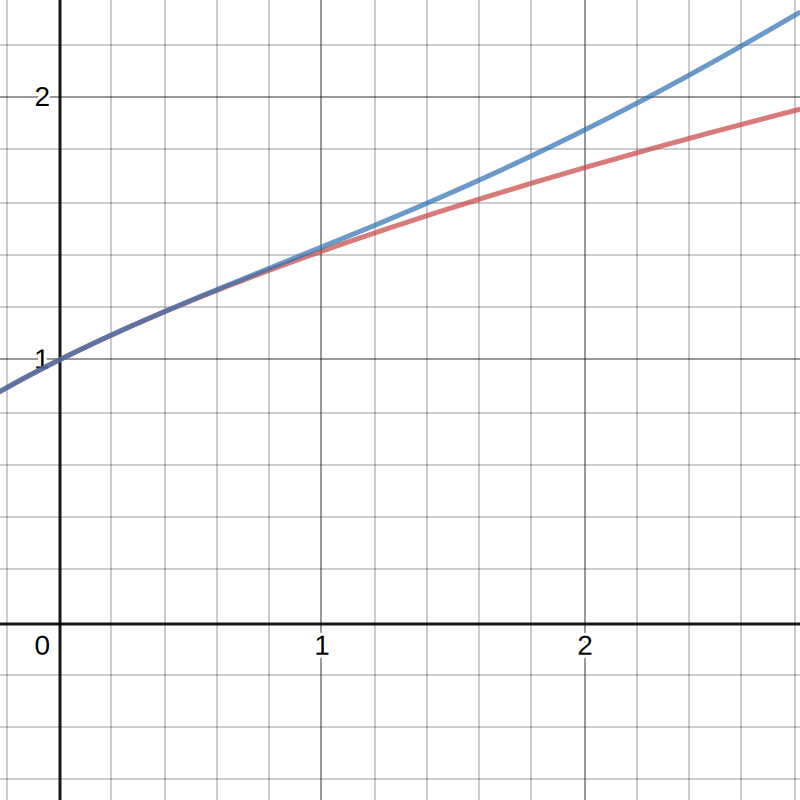
\includegraphics[width=0.5\textwidth]{desmos-graph.pdf}
		\caption{График функции и её разложения}\label{taylor-graph}
	\end{figure}


Ключ к приближению Френеля состоит в том, чтобы предположить, что третий член разложения очень мал и может быть проигнорирован, а с этого момента и более высоких порядков. Чтобы сделать это возможным, он должен вносить вклад в вариацию экспоненты для почти нулевого члена. Другими словами, он должен быть намного меньше периода комплексной экспоненты, то есть $2\pi$:
\begin{equation}
	k\frac{\rho^4}{8z^3}\ll 2\pi, \quad \frac{2\pi}{\lambda}\frac{\rho^4}{8z^3}\ll 2\pi, \quad\rho^4 \ll 8z^3\lambda \vline \times \frac{1}{\lambda^4}\quad\Rightarrow \quad\left(\frac{\rho}{\lambda}\right)^4 \ll 8\left(\frac{z}{\lambda}\right)^3
\end{equation}

Обычно длина волны много меньше физических размеров, особенно $z$. Таким образом, можем аппроксимировать \eqref{r} следующим образом
\begin{multline}
	r\approx z+\frac{\rho^2}{2z}=z+\frac{\left({x_i-x_0}\right)^2+\left({y_i-y_0}\right)^2}{2z}\Rightarrow \\
	\Rightarrow \ee{ikr} = \ee{ik\left(z+\frac{\left({x_i-x_0}\right)^2+\left({y_i-y_0}\right)^2}{2z}\right)}
\end{multline}
\subsubsection{Амплитудный член}\label{amplituda}
В параграфе \rbf{analiz} было получено, что экспоненциальный член обладает большим порядком роста, нежели амплитудный, поэтому его точность должна превалировать над точностью амплитудного члена. Таким образом, для амплитудного члена будет достаточно аппроксимации первого порядка, то есть 
\begin{equation}
	r \approx z \quad \Rightarrow \quad A(x_0, x_i) = \frac{1}{i\lambda z}
\end{equation}
\subsubsection{Итог}
Несмотря на то, что выведенные в параграфах \rbf{faza} и \rbf{amplituda} ограничения на соотношения размера окна, микрозазора и длины волны зачастую нарушаются в реальных процессах микролитографии, получаемые распределения весьма близки к экспериментальным результатам. На анимации \rbf{difference} приводится сравнение дифракционной картины, полученной при помощи различных уравнений в зависимости от величины микрозазора. 
\begin{center}
	\framebox{\textit{Нажмите $\triangleright$  для воспроизведения и $\parallel$ для остановки}}
\end{center}

%\includegraphics[width=0.5\textwidth]{animate/ani-0.png}
\begin{figure}[H]
	\centering
	\animategraphics[loop,controls={play,step},width=0.8\textwidth]{24}{animate/ani-}{0}{200}
	\caption{Сравнение дифракционной картины, полученной с помощью уравнения Рэлея-Зоммерфельда, (параксиального) приближения Френеля и (дальнего поля) приближения Фраунгофера.}\label{difference}
\end{figure}

\section{Программное обеспечение}
\subsection{Запуск Matlab}
\includegraphics[width=0.9\textwidth]{zapusk.png}
\subsection{Алгоритм расчёта, листинг программы}
Ниже приведён код программы с комментариями. Методика расчёта: задать массив $X$, в котором содержатся координаты границ отрезков разбиения. Затем проходимся циклом по этому массиву и вычисляем значения пределов интегрирования, интегралов Френеля и значений интенсивности в каждой точке. Записываем значения интенсивности $i$ в массив $I$. Выводим значения в .csv файл. После этого строим график из значений $X$ и $I$
   \includepdf[pages=-]
   {print.pdf} 
\subsection{Методика расчёта}
После выполнения программы получили график распределения интенсивности по координате, а также файл со значениями, несколько из которых приведены ниже
	\begin{figure}[H]
		\centering
		\includegraphics[trim=40 70 50 70,clip,width=0.9\textwidth]{untitled.pdf}
		\caption{График распределения интенсивности}\label{grafik}
	\end{figure}
	\begin{table}[H]
		
		\begin{center}
	\begin{tabular}{|c|c|c|c|c|c|c|c|}
		\hline
		$\xi_1$ & 		$\xi_2$ & $C_1$ & $C_2$ & $S_1$ & $S_2$ & $i$& $x$\\
		\hline
		3.9862& 11.9586& 0.4847& 0.4734& 0.4217& 0.4997& 0.0031& -3.0000\\
		\hline
		3.9543& 11.9267& 0.4552& 0.4900& 0.4332& 0.5247& 0.0048& -2.9880\\
		\hline
		3.9224& 11.8948& 0.4324& 0.5193& 0.4552& 0.5185& 0.0058& -2.9760\\
		\hline
		$\ldots$ &$\ldots$ &$\ldots$ &$\ldots$ &$\ldots$ &$\ldots$ &$\ldots$ &$\ldots$ \\
		\hline
		
	\end{tabular}
\end{center}\caption{Таблица результатов расчёта}
	\end{table}
\section{Иллюстрации}
\subsection{Расчётная схема}
\begin{center}
	\includegraphics[trim = 0 80 70 0,clip, width=0.7\textwidth]{scheme.jpg}
\end{center}
\subsection{Входное распределение интенсивности}
Показано на рис. \rbf{grafik} красной пунктирной линией $I_o$ и на рис. \rbf{vhod}
\begin{center}
	\begin{figure}[H]
		\centering
		\includegraphics[trim=0 185 220 0,clip,width=0.6\textwidth]{vhod.jpg}
		\caption{Профиль распределения излучения на шаблоне}\label{vhod}
	\end{figure}
\end{center}

\subsection{Профиль распределения интенсивности}
Приведён на рис. \rbf{grafik}
\end{document}